\documentclass{standalone}

\usepackage{xcolor}
\ifdefined\blue
  \definecolor{drawcolor}{HTML}{1E40AF}
  \definecolor{weakcolor}{HTML}{60A5FA}
\else
\ifdefined\dark
  \definecolor{drawcolor}{HTML}{cfcfcf}
  \definecolor{weakcolor}{HTML}{8f8f8f}
\else
\ifdefined\favicon
  \definecolor{drawcolor}{HTML}{ffffff}
  \definecolor{weakcolor}{HTML}{ffffff}
\else
  \definecolor{drawcolor}{HTML}{000000}
  \definecolor{weakcolor}{HTML}{505050}
\fi
\fi
\fi

\usepackage{tikz}
\usetikzlibrary{calc}

\usepackage[sfdefault]{quattrocento}
\usepackage[T1]{fontenc}

\tikzstyle{reverseclip}=[insert path={(current page.north east) --
  (current page.south east) --
  (current page.south west) --
  (current page.north west) --
  (current page.north east)}
]

\begin{document}

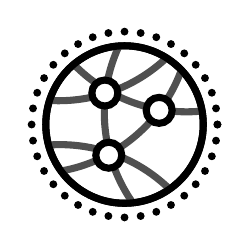
\begin{tikzpicture}[
  anchor=west, outer sep=0pt,
  line width=0.9mm,
  drawcolor,
  node/.style={anchor=center, line width=0.9mm, inner sep=0pt, circle, draw, minimum size=3.3mm},
]

  \ifdefined\favicon\else
    \foreach \d in {0, 10, ..., 360}
      \draw[fill=drawcolor, draw=none] (\d:1.18) circle (0.5mm);
  \fi

  \coordinate (p1) at (-0.25, 0.4);
  \coordinate (p2) at (0.44, 0.18);
  \coordinate (p3) at (-0.20, -0.39);

  \begin{scope}
    \draw (0, 0) circle (1);
    \clip (0, 0) circle (1);
    \ifdefined\favicon\else
      \clip (p1) circle (2mm) [reverseclip];
      \clip (p2) circle (2mm) [reverseclip];
      \clip (p3) circle (2mm) [reverseclip];
    \fi

    \draw[draw=weakcolor] (5:1.75) circle (2);
    \draw[draw=weakcolor] (130:1.8) circle (2);
    \draw[draw=weakcolor] (70:2.3) circle (2);
    \draw[draw=weakcolor] (110:2.45) circle (2);
    \draw[draw=weakcolor] (250:2.4) circle (2);
  \end{scope}

  \ifdefined\favicon\else
    \node[node] (r1) at (p1) {};
    \node[node] (r2) at (p2) {};
    \node[node] (r3) at (p3) {};
  \fi


  \draw (0, 0) circle (1);

  \ifdefined\text
    \node[right] at (1.3, 0) {\huge \bfseries BGP\,Sim};
  \fi
\end{tikzpicture}
\end{document}
